\documentclass[12pt]{article}
\usepackage{float}
\usepackage[table,xcdraw]{xcolor}
\usepackage{tikzit}
\input{Homework.tikzstyles}
\usepackage{hyperref}
\usepackage{amsmath}
\usepackage{amsfonts}
\usepackage{amssymb}
\usepackage{amsthm}
\usepackage{graphics}
\usepackage{graphicx}
\usepackage{yfonts}
\usepackage{float}
\usepackage{dsfont}
\usepackage[nottoc]{tocbibind}
\setcounter{tocdepth}{3}
\setcounter{secnumdepth}{3}
\usepackage{url}
\usepackage{multirow}
\usepackage{subcaption}
\usepackage{ctable}
\usepackage{caption}
\usepackage{pifont}
\usepackage{array}
\usepackage{adjustbox}
\usepackage{booktabs}
\usepackage{tabularx, booktabs, makecell, caption}
\usepackage{siunitx}
\usepackage{booktabs}
\captionsetup{labelformat=empty,labelsep=none}

\title{\textbf{\Luge Gastrointestinal Polyp Segmentation}\\[1ex] Use Encoder-Decoder Networks for Gastrointestinal Polyp Segmentation}
\author{\Large{ Mohammad Zamani}  \\ \Large{Student No. 610399135} \\ \\ \Large{University of Tehran- CS Department}}
\date{}

\usepackage{titling}
\renewcommand\maketitlehooka{\null\mbox{}\vfill}
\renewcommand\maketitlehookd{\vfill\null}

\begin{document}
	%%%%%%%%%%%%%%%%%%%%%       Title Page      %%%%%%%%%%%%%%%%%%%%%%		

	
	\begin{titlingpage}
	
	\begin{figure}
		\centering
		
\includegraphics[width=0.3\textwidth]{Figs/University_of_Tehran_logo.png}		
	\end{figure}		\maketitle
	
	\end{titlingpage}
		
	


	%%%%%%%%%%%%%%%%%%%%%       Page 1       %%%%%%%%%%%%%%%%%%%%%%

	\setlength{\parindent}{20pt}
	\tableofcontents
	
	\vspace{1\baselineskip}

	\pagebreak
	\section{Abstract}

	Detecting abnormal tissues can be overlooked during body screening procedures including endoscopy, bronchoscopy, and colonoscopy. Colonoscopy is a routine screening procedure that can examine inside of the large intestine. However, observants might not be able to detect anomalies at initial phase. Therefore, a precise method is needed to detect the abnormalities. in this project we want to use  some pretrained different convolutional neural networks with different encoders and decoders to segment polyps in gastrointestinal tract images, we will test and evaluate some models like UNET, UNET++, DeepLab and PSPNet with different encoders and finally combine them to reach state-of-the-art performance results.

	\section{Introduction}
	
	Colorectal cancer is one of the most common malignancies of the digestive tract and a leading cause of cancer-related death in both sexes. Polyps are abnormal growths of tissue from the mucous membrane. Colorectal polyps are usually benign, while some might be precancerous or even cancerous over a period of 5 to 15 years. Colorectal polyps can become lethal in their later stages. Therefore, it is critical to detect and remove them at an earlier stage.

Developments in computer vision and artificial intelligence algorithms have influenced various fields of science and industry. They have simplified the most complicated problems encountered in a wide variety of professions, including engineering, art, and medicine. The trend shows an increasing demand for the use of automation for a variety of tasks in real operations.

The idea behind image segmentation is to assign the same label to pixels that have the same specific characteristics. Image segmentation and object detection techniques can divide an image into meaningful parts that are easier to analyze and interpret. Image segmentation techniques can assist in detecting abnormalities in medical images. These techniques can aid pathologists in many ways, such as monitoring and improving diagnostic ability. In this paper, we have experimented with eight different architectures: UNet, UNet++, DeepLab, and PSPNet, with ResNet50 and MobileNetV2 as encoders for polyp segmentation to decrease the chance of polyps being overlooked.


	\section{Methodology}
	
	\subsection{Methods}
	The major steps in this project involved familiarizing ourselves with the Kvasir-SEG dataset, preprocessing the polyp and mask images, selecting and combining models, training, and evaluating the results.

	\subsection{Dataset}
	The Kvasir-SEG dataset (size 46.2 MB) contains 1000 polyp images and their corresponding ground truth from the Kvasir Dataset v2. The resolution of the images contained in Kvasir-SEG varies from $332 \times 487$ to $1920 \times 1072$ pixels. The images and its corresponding masks are stored in two separate folders with the same filename. The image files are encoded using JPEG compression, and online browsing is facilitated. The open-access dataset can be easily downloaded for research and educational purposes.


\begin{figure}[H]
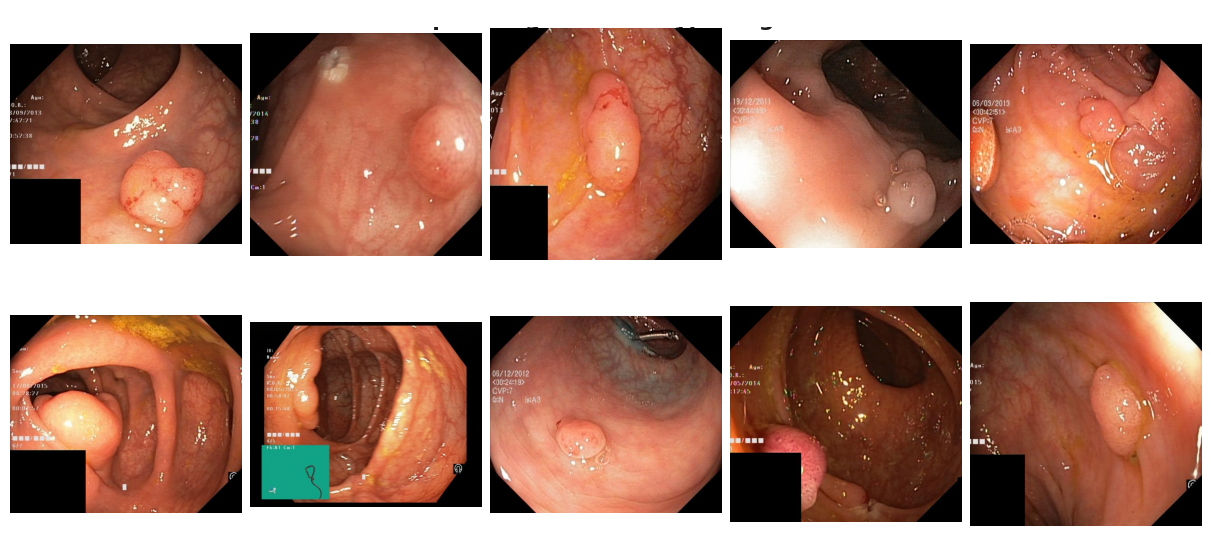
\includegraphics[width=1\textwidth]{Figs/Kvasir-SEG-sample.png}
\caption{Fig2. Polyp samples}
\label{fig:Dataset}
\end{figure}
	
	\subsection{Encoders}
	
	The encoder subnetwork takes an input image and compresses it into a lower-dimensional representation, also known as a latent space. This process involves passing the input image through multiple layers of convolution and pooling operations, which gradually reduce the spatial dimensions of the image while extracting important features Fig.\ref{fig:encoder}. In our models for implementing encoder-decoder networks, we should pick an appropriate encoder. We use some popular pre-trained encoders.
	
\begin{center}
\begin{figure}[H]
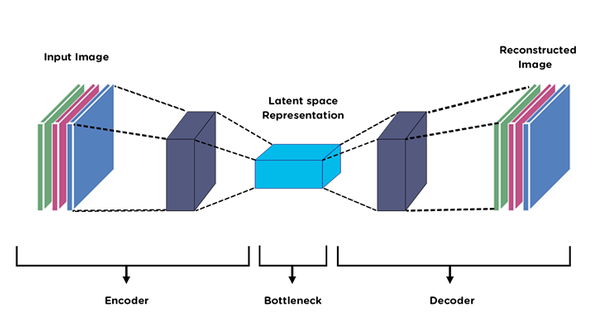
\includegraphics[width=1\textwidth]{Figs/encoder-decoder.png}
\caption{Fig.2 Encoder And Decoder Structure}
\label{fig:encoder}
\end{figure}
\end{center}
	
	\subsubsection{MobileNet V2}
		MobileNet  was  created  by  Google  and  has  a  special layer called depthwise  separable  convolution,  which  is a   block   consisting   of   depthwise   convolution   and pointwise  convolution.  The  purpose  of  this  layer  is  to reduce computation (to have  fewer parameters)  so that a  smaller  model  size  can  be  obtained.  MobileNet is  a  small,  low-latency,  low-power  model  measured  to meet  the  resource  constraints  of  various  use  cases. According  to  research  papers,  MobileNetv2  improves the  performance  of  advanced  mobile  models  on  many tasks  and  benchmarks  as  well  as  across  the  entire spectrum  of  different  model  sizes.  MobileNetv2  is  a highly  effective  feature  extractor  for  object  detection and segmentation.
	
	
	\subsubsection{Resnet50}
	
	The ResNet50 is made up of 5 convolutional blocks on the 5 consecutive sizes of the encoding part. Each block is implemented via the Residual module that learns the difference between the input and the output of the block. This residue is obtained by passing the input value through 2 or 3 convolutional layers. the key innovation of ResNet (Residual Networks) lies in its use of residual connections, also known as skip connections. These skip connections allow the network to bypass one or more layers, enabling the flow of information directly from earlier layers to later layers. This addresses the vanishing gradient problem, which can occur in very deep neural networks during training. By using skip connections, ResNet enables the network to learn residual mappings instead of directly learning the desired underlying mapping. This approach facilitates the training of much deeper networks while still maintaining good performance. As a result, ResNet architectures have been highly successful in various computer vision tasks, such as image classification, object detection, and semantic segmentation.


	
	\subsection{Docoders}	
	
	\subsubsection{U-Net}
	before UNET we used a common fully convolutional network, Fig.\ref{fig:beforeUNET} shows this model structure.
	
\begin{center}
\begin{figure}[H]
\centering
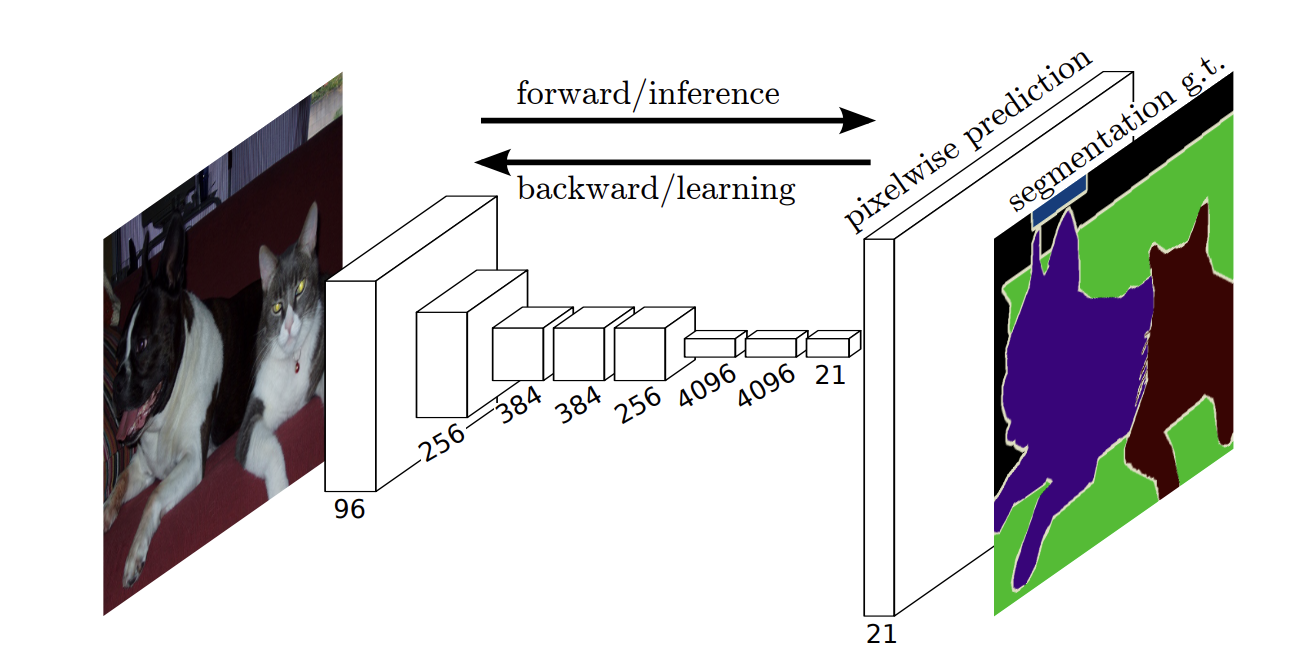
\includegraphics[width=0.8\textwidth]{Figs/beforeUNET}
\caption{Fig.3  Fully convolutional networks can efficiently learn to make dense predictions for perpixel tasks like semantic segmentation.}
\label{fig:beforeUNET}
\end{figure}
\end{center}
	
	UNET modify and extend this architecture such that it works with very few training images and yields more precise segmentations. The main idea in \ref{fig:beforeUNET} is to supplement a usual contracting network by successive layers, where pooling operators are replaced by upsampling operators. Hence, these layers increase the resolution of the output. In order to localize, high
resolution features from the contracting path are combined with the upsampled output. A successive convolution layer can then learn to assemble a more precise output based on this information. One important modification in UNET architecture is that in the upsampling
part and UNET have also a large number of feature channels, which allow the network
to propagate context information to higher resolution layers. As a consequence,
the expansive path is more or less symmetric to the contracting path, and yields
a u-shaped architecture. The network does not have any fully connected layers
and only uses the valid part of each convolution, i.e., the segmentation map only
contains the pixels, for which the full context is available in the input image.
This strategy allows the seamless segmentation of arbitrarily large images by an
overlap-tile strategy.
	
	
	
	\subsubsection{U-Net++}
	UNet++ introduces the concept of nested skip pathways to bridge this semantic gap. It adds additional skip connections between the encoder and decoder blocks at multiple resolutions. These connections allow the decoder to access and incorporate both low-level and high-level features from the encoder, providing a more detailed and comprehensive understanding of the image.  UNet++ improved the traditional U-Net architecture by redesigning the skip connections and introducing a deeply supervised nested encoder-decoder network. The key difference between UNet and UNet++ lies in the architecture: UNet++ extends UNet by introducing nested skip pathways and dense skip connections, enabling more effective multi-scale feature aggregation and potentially improving segmentation accuracy.
	
	\subsubsection{PSPNet}
	The key idea and innovation behind PSPNet (Pyramid Scene Parsing Network) lie in the use of pyramid pooling modules to capture contextual information at multiple scales effectively. PSPNet's incorporates pyramid pooling modules, which divide the feature maps into fixed-size grids and pool features from each grid separately. By doing so, PSPNet captures contextual information at multiple scales, enabling it to better understand the global context of the scene while preserving fine-grained details. This approach enhances the network's ability to parse scenes accurately, especially in complex scenes with objects of various scales. Fig.\ref{fig:PSPNet} Shows an overview of PSPNet.
 	
\begin{center}
\begin{figure}[H]
\centering
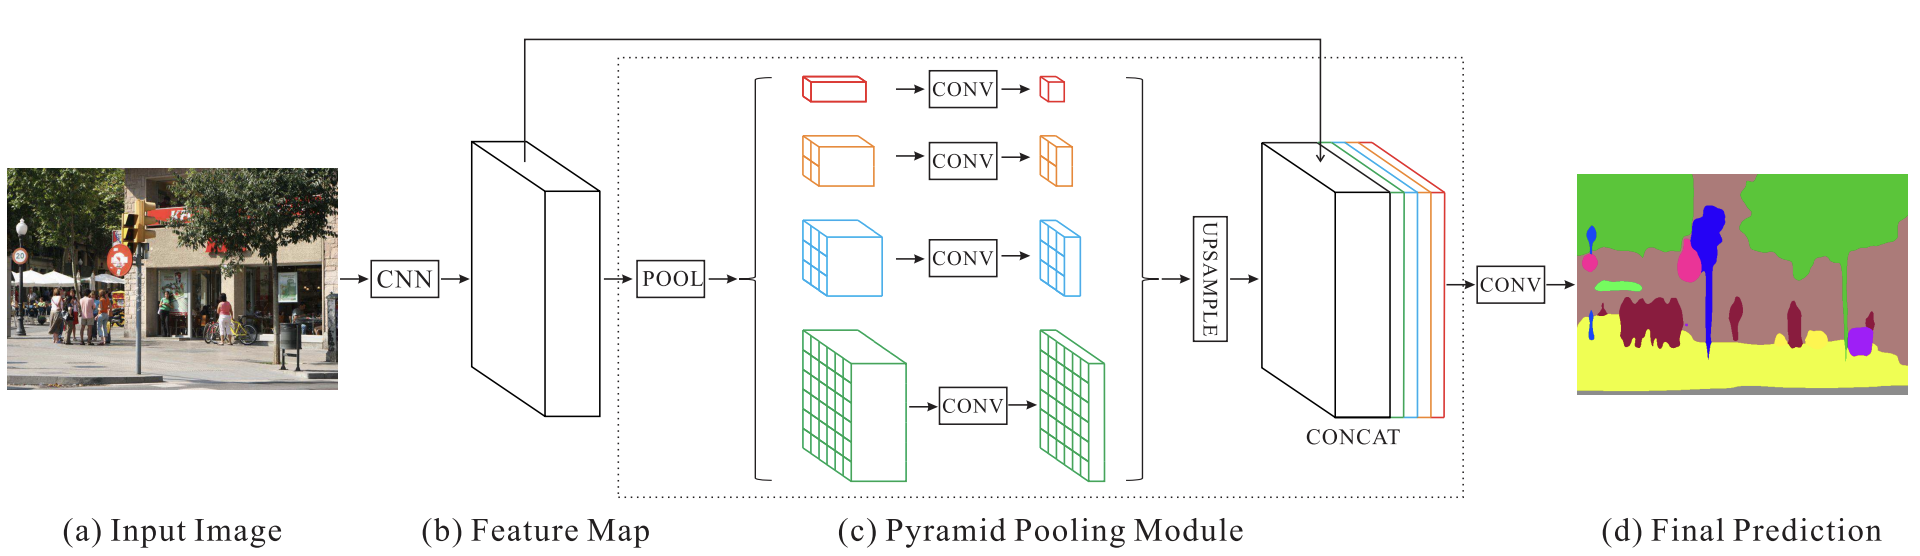
\includegraphics[width=1\textwidth]{Figs/PSPNet}
\caption{Fig.4 . Overview of PSPNet. Given an input image (a), we first use CNN to get the feature map of the last convolutional layer (b), then a pyramid parsing module is applied to harvest different sub-region representations, followed by upsampling and concatenation layers to form the final feature representation, which carries both local and global context information in (c). Finally, the representation is fed into a convolution layer to get the final per-pixel prediction (d).}
\label{fig:PSPNet}
\end{figure}
\end{center}
	
	\subsubsection{DeepLabV3Plus}	
	DeepLabV3Plus achieves state-of-the-art semantic segmentation performance by leveraging atrous convolutions, encoder-decoder architecture with skip connections, and spatial pyramid pooling to effectively capture multi-scale contextual information while preserving spatial details.
	
	
	\subsection{Transfer learning}
	
	Deep convolutional neural network models may take days or even weeks to train on very large datasets.
A way to shortcut this process is to reuse the model weights from pre-trained models developed for standard computer vision benchmark datasets, such as the ImageNet image recognition tasks. Top-performing models can be downloaded and used directly or integrated into a new model for your own computer vision problems.
In this project, I'll be using the UNet, UNet++, PSPNet, and DeepLabV3Plus architectures, with ResNet50 and MobileNet serving as encoders, to construct eight different encoder-decoder networks. These networks will leverage pre-trained weights from the ImageNet dataset.



	\section{Results}
	\subsection{Metrics}
	
	\subsubsection{Dice Score}
	This competition is evaluated on the mean Dice coefficient. The Dice coefficient can be used to compare the pixel-wise agreement between a predicted segmentation and its corresponding ground truth. The formula is given by:
	
	\begin{equation}
	\frac{2 \times |X \cap Y |}{|X| + |Y|}
	\end{equation}
	
	where X is the predicted set of pixels and Y is the ground truth. The Dice coefficient is defined to be 1 when both X and Y are empty. The leaderboard score is the mean of the Dice coefficients for each image in the test set.
	
	In summary, the Dice score operates similarly to the F1-Score, measuring the agreement between predicted and ground truth regions. To normalize the score, we add 2 to the numerator. Figure \ref{fig:DiceScore} illustrates the Dice score in its simplest form.

\begin{figure}[H]
\centering
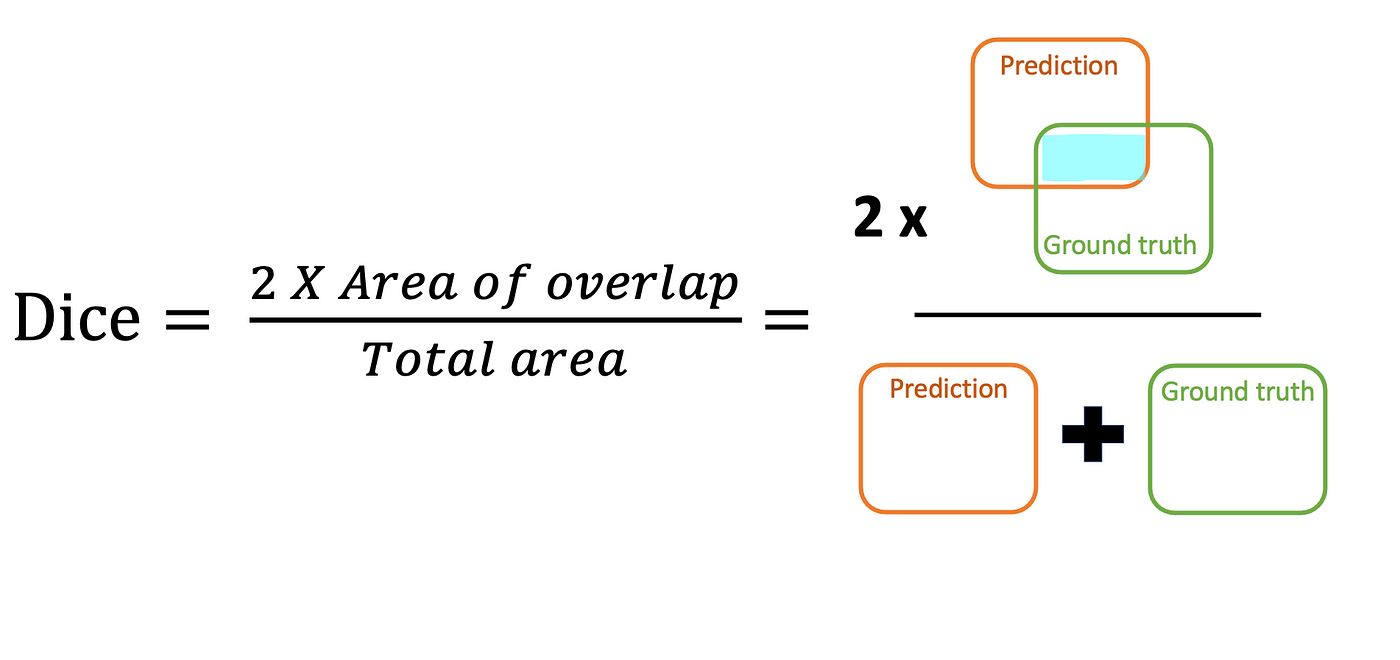
\includegraphics[width=0.65\textwidth]{Figs/DiceScore}
\caption{Fig.5 Dice Score}
\label{fig:DiceScore}
\end{figure}
\end{center}


	\subsubsection{Dice Loss}
	Dice Loss is complement of Dice Score, So if you minimize the Dice loss you are maximizing Dice Score I used it as my loss function in training.
	\begin{equation}
	Dice-Loss = 1 - Dice-Score
	\end{equation}
	
	\subsubsection{IOU Score}	
	IOU is calculated by dividing the area of intersection between the predicted and ground truth regions by the area of their union. The formula for IOU can be expressed as follows:
	
	\begin{equation}
		\frac{2 \times |X \cap Y |}{|X \cup Y|}
	\end{equation}
	A higher IOU value indicates a better alignment between the predicted and actual regions, reflecting a more accurate model. Figure \ref{fig:IOUScore} illustrates the Dice score in its simplest form.
	
\begin{figure}[H]
\centering
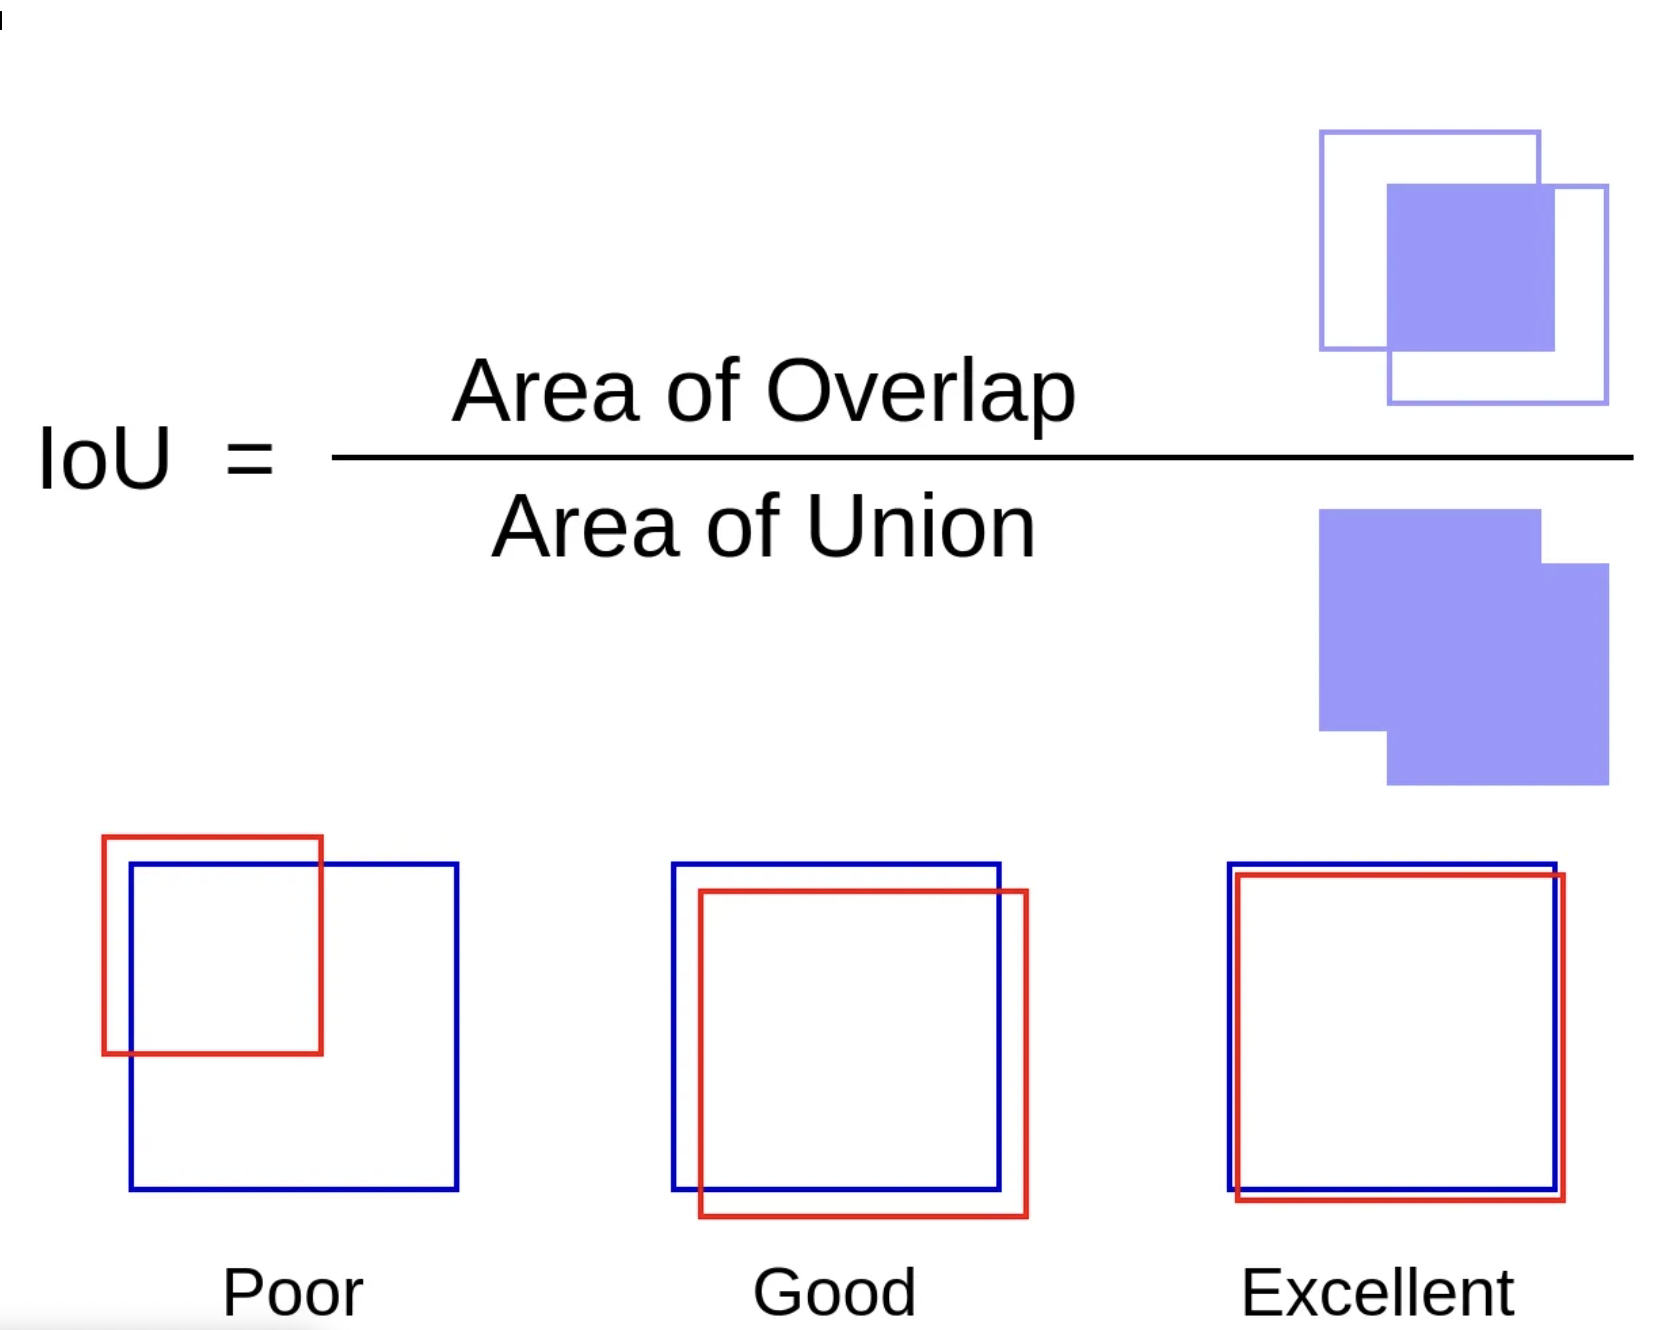
\includegraphics[width=0.7\textwidth]{Figs/iouscore}
\caption{Fig.6 IOU Score}
\label{fig:IOUScore}
\end{figure}
\end{center}
	
	
	\subsection{Training Results}
	In this section, I will visualize the Dice Loss and IoU score for each model across training epochs to depict the training process of each model.


\begin{figure}[H]
  \begin{subfigure}[b]{0.5\textwidth}
    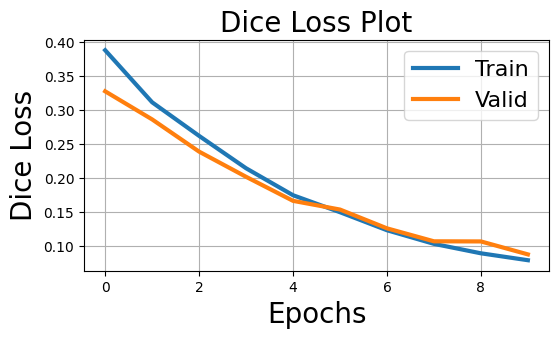
\includegraphics[width=\textwidth]{Figs/unetwithresnetdice.png}
    \caption{Dice Loss}
    \label{fig:f1}
  \end{subfigure}
  \hfill
  \begin{subfigure}[b]{0.5\textwidth}
    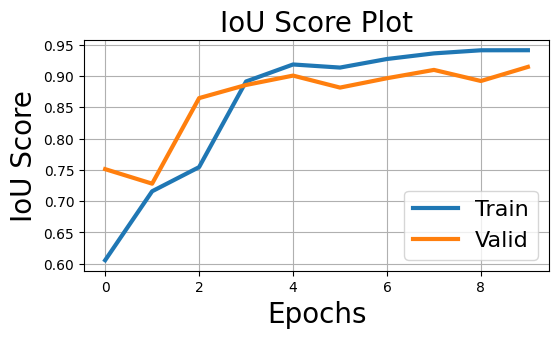
\includegraphics[width=\textwidth]{Figs/unetwithresnetiou.png}
    \caption{IoU Score}
    \label{fig:f2}
  \end{subfigure}
  \caption{Unet With Resnet50}
\end{figure}


\begin{figure}[H]
  \begin{subfigure}[b]{0.5\textwidth}
    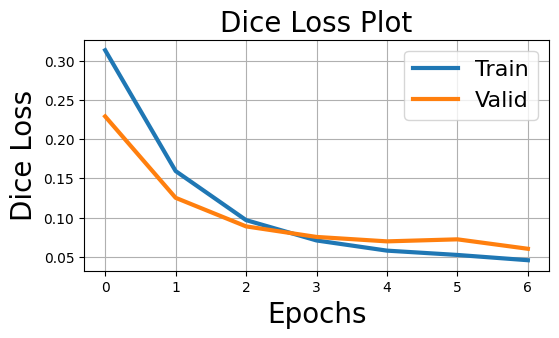
\includegraphics[width=\textwidth]{Figs/unetwithmbnetdice.png}
    \caption{Dice Loss}
    \label{fig:f1}
  \end{subfigure}
  \hfill
  \begin{subfigure}[b]{0.5\textwidth}
    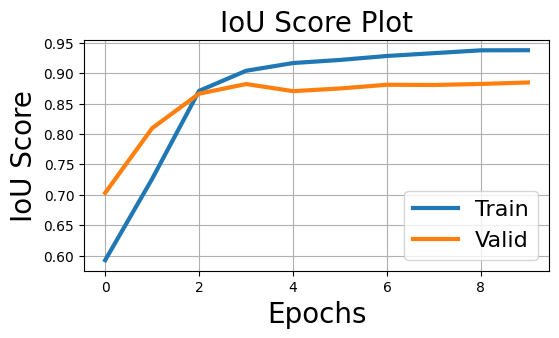
\includegraphics[width=\textwidth]{Figs/unetwithmbnetiou.png}
    \caption{IoU Score}
    \label{fig:f2}
  \end{subfigure}
  \caption{Unet With MobileNetV2}
\end{figure}

\begin{figure}[H]
  \begin{subfigure}[b]{0.5\textwidth}
    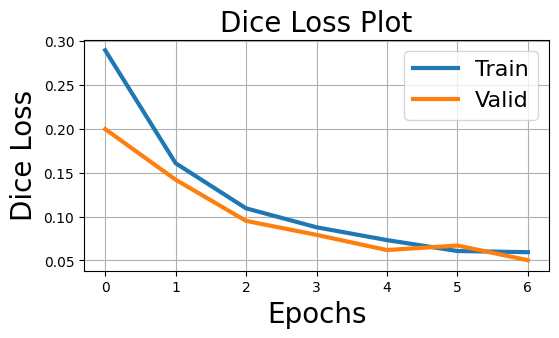
\includegraphics[width=\textwidth]{Figs/unet++withresnetdice.png}
    \caption{Dice Loss}
    \label{fig:f1}
  \end{subfigure}
  \hfill
  \begin{subfigure}[b]{0.5\textwidth}
    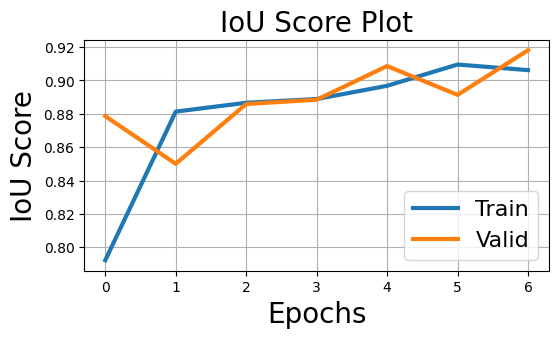
\includegraphics[width=\textwidth]{Figs/unet++withresnetiou.png}
    \caption{IoU Score}
    \label{fig:f2}
  \end{subfigure}
  \caption{Unet++ With Resnet50}
\end{figure}

\begin{figure}[H]
  \begin{subfigure}[b]{0.5\textwidth}
    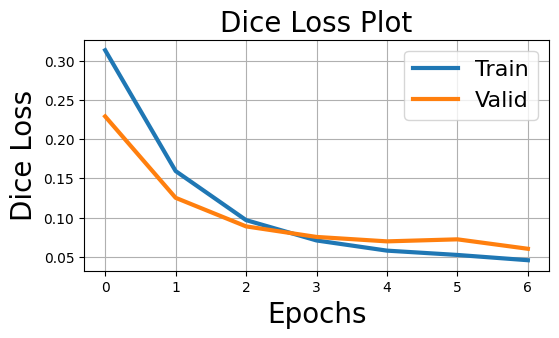
\includegraphics[width=\textwidth]{Figs/unet++withmbnetdice.png}
    \caption{Dice Loss}
    \label{fig:f1}
  \end{subfigure}
  \hfill
  \begin{subfigure}[b]{0.5\textwidth}
    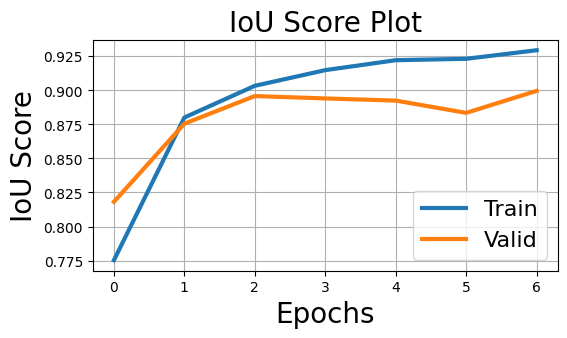
\includegraphics[width=\textwidth]{Figs/unet++withmbnetiou.png}
    \caption{IoU Score}
    \label{fig:f2}
  \end{subfigure}
  \caption{Unet++ With MobileNetV2}
\end{figure}

\begin{figure}[H]
  \begin{subfigure}[b]{0.5\textwidth}
    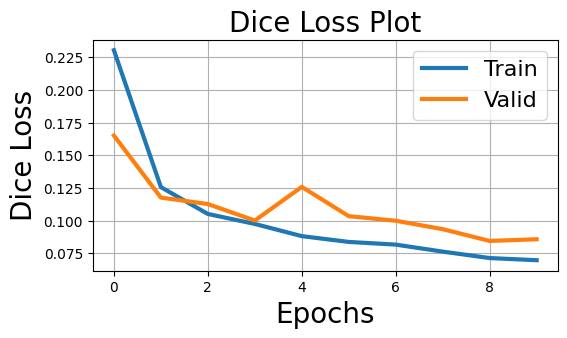
\includegraphics[width=\textwidth]{Figs/pspnetwithresnetdice.png}
    \caption{Dice Loss}
    \label{fig:f1}
  \end{subfigure}
  \hfill
  \begin{subfigure}[b]{0.5\textwidth}
    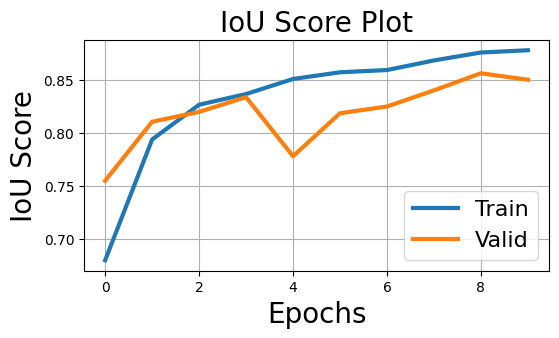
\includegraphics[width=\textwidth]{Figs/pspnetwithresnetiou.png}
    \caption{IoU Score}
    \label{fig:f2}
  \end{subfigure}
  \caption{PSPNet With Resnet50}
\end{figure}

\begin{figure}[H]
  \begin{subfigure}[b]{0.5\textwidth}
    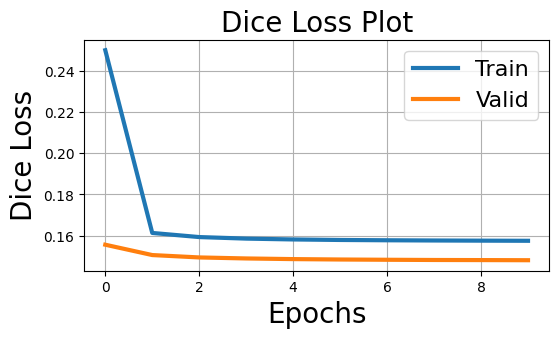
\includegraphics[width=\textwidth]{Figs/pspnetwithmbnetdice.png}
    \caption{Dice Loss}
    \label{fig:f1}
  \end{subfigure}
  \hfill
  \begin{subfigure}[b]{0.5\textwidth}
    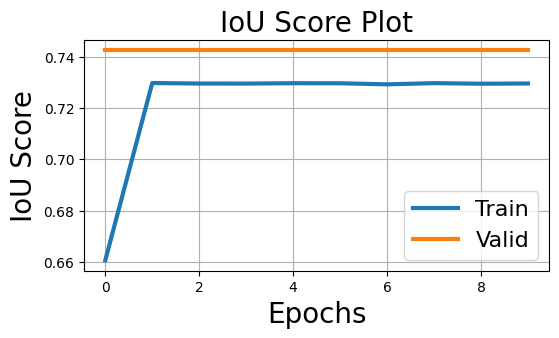
\includegraphics[width=\textwidth]{Figs/pspnetwithmbnetiou.png}
    \caption{IoU Score}
    \label{fig:f2}
  \end{subfigure}
  \caption{PSPNet With MobileNetV2}
\end{figure}


\begin{figure}[H]
  \begin{subfigure}[b]{0.5\textwidth}
    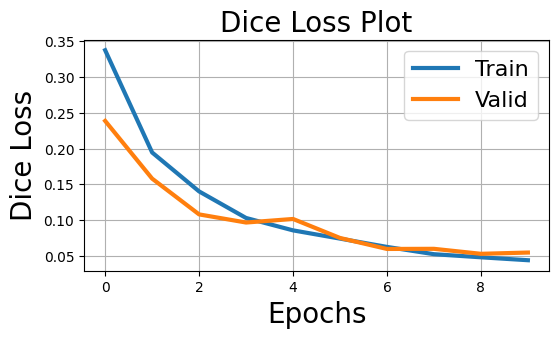
\includegraphics[width=\textwidth]{Figs/deepwithresnetdice.png}
    \caption{Dice Loss}
    \label{fig:f1}
  \end{subfigure}
  \hfill
  \begin{subfigure}[b]{0.5\textwidth}
    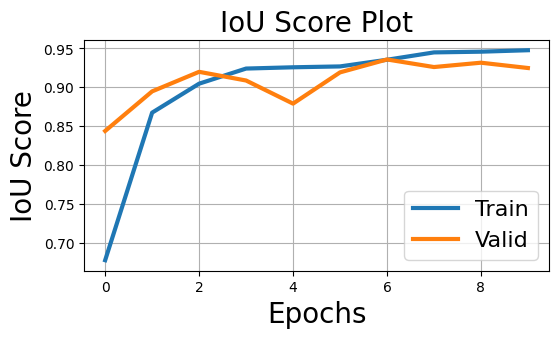
\includegraphics[width=\textwidth]{Figs/deepwithresnetiou.png}
    \caption{IoU Score}
    \label{fig:f2}
  \end{subfigure}
  \caption{DeepLabV3Plus With Resnet50}
\end{figure}

\begin{figure}[H]
  \begin{subfigure}[b]{0.5\textwidth}
    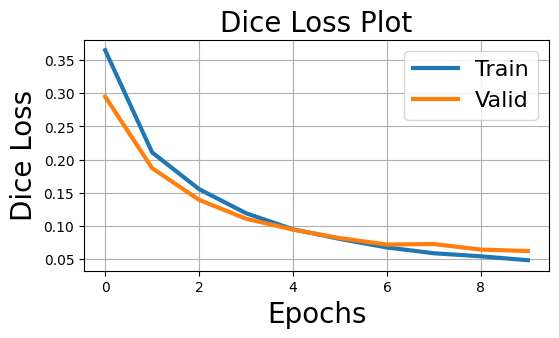
\includegraphics[width=\textwidth]{Figs/deepwithmbnetdice.png}
    \caption{Dice Loss}
    \label{fig:f1}
  \end{subfigure}
  \hfill
  \begin{subfigure}[b]{0.5\textwidth}
    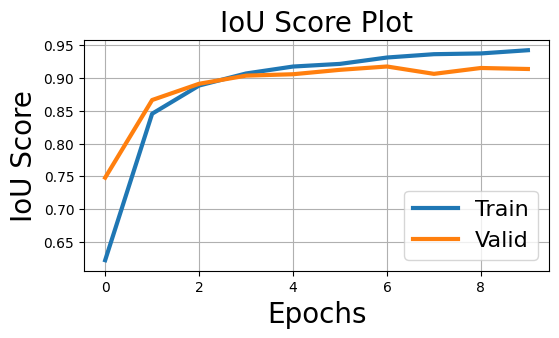
\includegraphics[width=\textwidth]{Figs/deepwithmbnetiou.png}
    \caption{IoU Score}
    \label{fig:f2}
  \end{subfigure}
  \caption{DeepLabV3Plus With MobileNetV2}
\end{figure}

We understand that optimal training occurs when both the training and validation losses decrease across epochs while minimizing the gap between them. Additionally, the training and validation scores should increase with minimal disparity. In several models, such a pattern is observable. However, there are instances, like in the case of PSPNet with MobileNetV2, where training might not proceed optimally, potentially leading to suboptimal model performance.

	\subsection{Test Results}
	And Finally I run my test set on models and you can see the final result in Table \ref{table:1}.

\begin{table}[H]
\centering
\begin{tabular}{@{}rrrrcrrr@{}}\toprule
& \multicolumn{3}{c}{$ResNet50$} & \phantom{abc}& \multicolumn{3}{c}{$MobileNetV2$}\\
\cmidrule{2-4} \cmidrule{5-7} 
\\
& $IoU$ & $DiceS$ & $DiceL$ && $IoU$ & $DiceS$ & $DiceL$ \\ \midrule

$UNet$ & 0.9261 & 0.9163 & 0.0837 && 0.9012 & 0.8972 & 0.1028\\
\\
$Unet++$ &  0.9229& 0.9495 & 0.0505 && 0.9086 & 0.9418 & 0.0582\\
\\
$PSPNet$ & 0.8652 &  0.9187 & 0.0813 && 0.7686 & 0.8586 & 0.1414\\
\\
$DeepLV3$ & 0.9064 & 0.9316 & 0.0684 && 00.9264 & 0.9429 & 0.0571\\
\\
\bottomrule
\end{tabular}
\caption{\textbf{Table 1.} Performance analysis of different combinations of pretrained encoders and decoders on the Kvasir databaset.}
\label{table:1}
\end{table}

Finally I plot the scores and losses for better visualization and reasoning.

\begin{figure}[H]
\centering
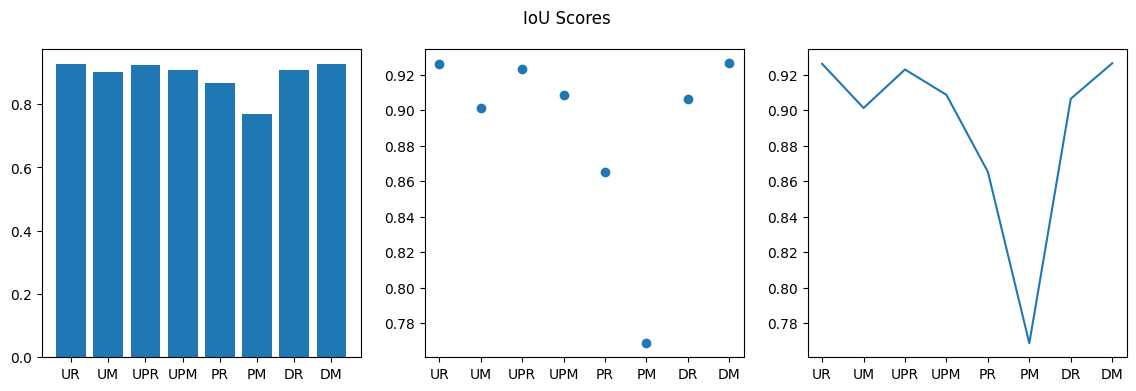
\includegraphics[width=1\textwidth]{Figs/resiou}
\caption{Fig.7 All Models IOU Scores}
\end{figure}
\end{center}

\begin{figure}[H]
\centering
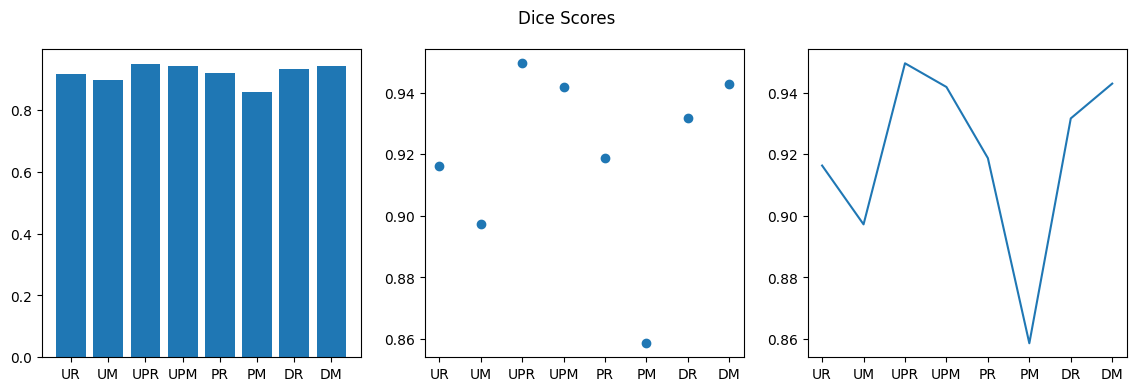
\includegraphics[width=1\textwidth]{Figs/resdice}
\caption{Fig.8 All Models Dice Scores}
\end{figure}
\end{center}

\begin{figure}[H]
\centering
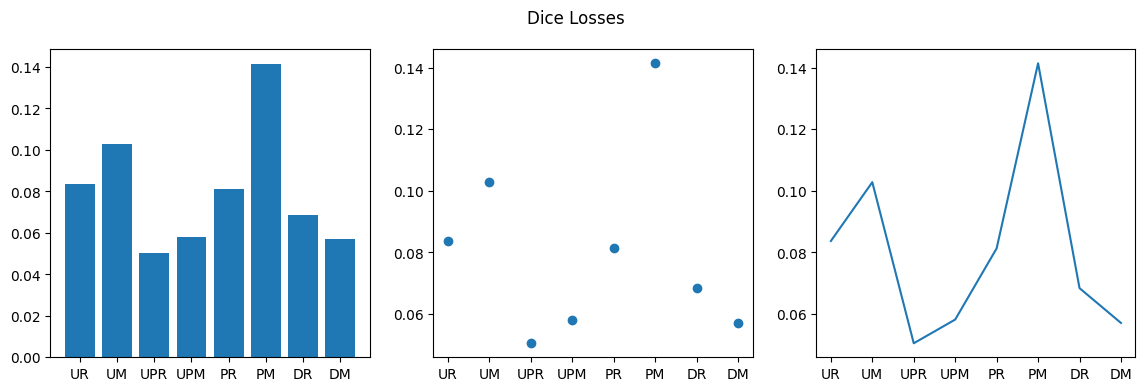
\includegraphics[width=1\textwidth]{Figs/resdicel}
\caption{Fig.9 All Models Dice Losses}
\end{figure}
\end{center}

	
	\section{Conclusion}
	In this project we have analyzed multiple decoder-encoder networks for the task of polyp segmentation on endoscopic images. we combine these models to gain best result and finally state-of-the-art-model for this task is UNet++ with ResNet50.

%%%%%%%%%%%%%%%%%%%%%%%%%%%%%%%%%%%%%%%%%%%%%%%%%%%%%%%%%%%%%%%%%%%%%%%%%%%%%%%%%%%%%%%%%%%%%%%

		%%%%%%%%%%%%%%%%    References    %%%%%%%%%%%%%%%%%%%
	
	
	\begin{thebibliography} {1} % Replace '9' with the widest label in your citations
		\bibitem{Double Encoder-Decoder Networks for Gastrointestinal Polyp Segmentation}Double Encoder-Decoder Networks for Gastrointestinal Polyp Segmentation. Adrian Galdran
, Gustavo Carneiro and Miguel A. Gonz ́alez Ballester. 5 Oct 2021.
		
		\bibitem{U-Net: Convolutional Networks for Biomedical
Image Segmentation } U-Net: Convolutional Networks for Biomedical
Image Segmentation. Olaf Ronneberger, Philipp Fischer, and Thomas Brox.  18 May 2015.
		
		\bibitem{Encoder-Decoder with Atrous Separable
Convolution for Semantic Image Segmentation}Encoder-Decoder with Atrous Separable
Convolution for Semantic Image Segmentation. Liang-Chieh Chen, Yukun Zhu, George Papandreou, Florian Schroff, and Hartwig Adam. Aug 22, 2018.
	
		\bibitem{Pyramid Scene Parsing Network} Pyramid Scene Parsing Network. Hengshuang Zhao,
Jianping Shi, Xiaojuan Qi, Xiaogang Wang,
Jiaya Jia, The Chinese University of Hong Kong 2SenseTime Group Limited. 27 Apr 2017
		
		\bibitem{ Fully Convolutional Networks for Semantic Segmentation}Fully Convolutional Networks for Semantic Segmentation. Jonathan Long, Evan Shelhamer, Trevor Darrell. 8 Mar, 2015.
		
		\bibitem{Segmentation of Polyps in Gastrointestinal Tract Images}Segmentation of Polyps in Gastrointestinal (GI) Tract Images. Sabrina Nasrin, Javaneh Alavi, Pamila Viswanathan. 23 Dec 2021.
		
		\bibitem{Image Segmentation of Normal Pap Smear Thinprep using U-Net with Mobilenetv2 Encoder} Image Segmentation of Normal Pap Smear Thinprep using U-Net with Mobilenetv2 Encoder. Deviana Sely Wita. 30June 23. 

	
	\bibitem{U-Net architecture variants for brain tumor segmentation of histogram corrected images} U-Net architecture variants for brain tumor segmentation of histogram corrected images. Sz. Lefkovits, L. Lefkovits. 2022.
	
	\bibitem{Encoder–Decoder Convolutional Neural Networks for Flow Modeling in Unsaturated Porous Media: Forward and Inverse Approaches} Encoder–Decoder Convolutional Neural Networks for Flow Modeling in Unsaturated Porous Media: Forward and Inverse Approaches. Mohammad Reza Hajizadeh Javaran. 14 July 2023 
	
	\bibitem{ CS231n: Convolutional Neural Networks for Visual Recognition} \href{https://cs231n.github.io/} CS231n: Convolutional Neural Networks for Visual Recognition
	
\end{document}